\breakpagebeforenextheadingtrue
\section{Implementation and Numerical Results}
\label{sec:73results}

\minitoc[0mm]{69mm}{8}

\parbox{1em}{}
\vspace{-3em}



\disableornamentsfornextheadingtrue
\subsection{Implementation}
\label{sec:731implementation}

\paragraph{Parameters, implementation, and geometry}

Details about implementational aspects of the model can be found in
\multicite{Sprenger15Continuum,Roehrle16Two,Valentin18Gradient},
for instance, values for the material parameters.
%
The constitutive law has been implemented in the CMISS software package
(an interactive computer program for Continuum Mechanics,
Image analysis, Signal processing and System identification%
\footnote{%
  \url{https://www.cmiss.org/}%
}).
The emerging PDEs are discretized using quadratic finite element basis
functions and the resulting linearized system is solved with CMISS.
%
The geometry of the human upper limb model is based on
the Visible Human Male's dataset \cite{Spitzer96Visible}.
Again, we refer to \multicite{Sprenger15Continuum,Roehrle16Two} for details
about the geometry.



\subsection{Reference and Sparse Grid Solution}
\label{sec:732solutionTypes}

\paragraph{Reference solution}

Since the model is only two-dimensional, we can compute a reference solution
on a full grid.
To this end, we evaluate the exerted muscle forces $\forceT$ and $\forceB$ on
the full grid
\begin{equation}
  \{\ang{10}, \ang{11}, \dotsc, \ang{150}\} \times \{0, 0.1, \dotsc, 1\}
  \ni (\elbang, \actX),\quad
  X \in \{\mathrm{T}, \mathrm{B}\}.
\end{equation}
The resulting \num{1551} grid points
are interpolated with bicubic full grid splines%
\footnote{%
  Computed with the Geometric Tools Engine \cite{Schneider03Geometric},
  see \url{https://www.geometrictools.com/}.%
}
to obtain \term{reference solutions}
$\forceTref, \forceBref\colon
\clint{\ang{10}, \ang{150}} \times \clint{0, 1} \to \real$,
which are shown in \cref{fig:biomech2ReferenceForce}.
Due to the high resolution of the full grid,
we may assume that the reference solutions are accurate enough
to ensure $\forceTref \approx \forceT$ and $\forceBref \approx \forceB$.
We refer to the resulting equilibrium elbow angle
with $\equielbangref{\forceL}$.
It is displayed in
\cref{fig:biomech2ReferenceEquilibriumAngle}
for the loads of $\forceL = \SI{22}{\newton}$,
$\SI{-60}{\newton}$, and $\SI{180}{\newton}$.

\begin{figure}
  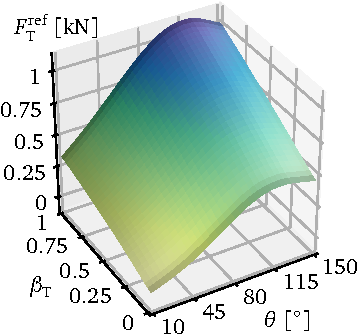
\includegraphics{biomech2ReferenceForce_1}%
  \;\;%
  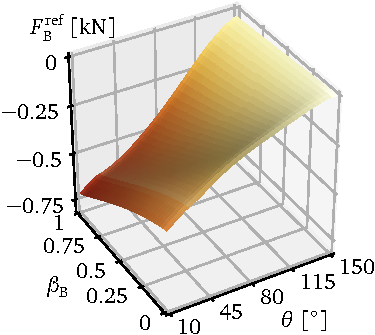
\includegraphics{biomech2ReferenceForce_2}%
  \hfill%
  \rlap{\raisebox{53mm}{\;$\forceXref$ [\si{\kilo\newton}]}}%
  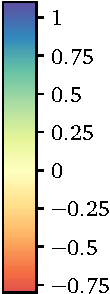
\includegraphics{biomech2ReferenceForce_3}%
  \caption[Reference triceps and biceps forces]{%
    Reference triceps and biceps forces $\forceXref$
    ($X \in \{\mathrm{T}, \mathrm{B}\}$).%
  }%
  \label{fig:biomech2ReferenceForce}%
\end{figure}

\begin{figure}
  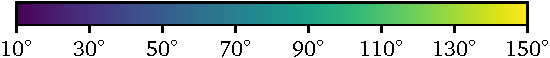
\includegraphics{biomech2ReferenceEquilibriumAngle_4}%
  \\[2mm]%
  \subcaptionbox{%
    $\forceL = \SI{22}{\newton}$%
  }[49mm]{%
    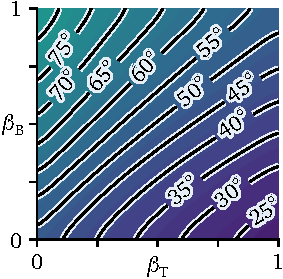
\includegraphics{biomech2ReferenceEquilibriumAngle_1}%
  }%
  \hfill%
  \subcaptionbox{%
    $\forceL = \SI{-60}{\newton}$%
  }[49mm]{%
    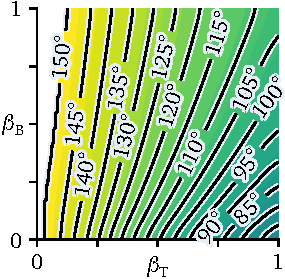
\includegraphics{biomech2ReferenceEquilibriumAngle_2}%
  }%
  \hfill%
  \subcaptionbox{%
    $\forceL = \SI{180}{\newton}$%
  }[49mm]{%
    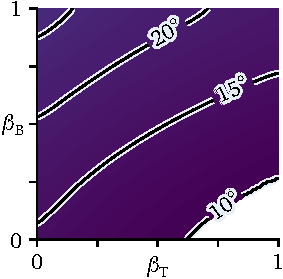
\includegraphics{biomech2ReferenceEquilibriumAngle_3}%
  }%
  \caption[Reference equilibrium elbow angle]{%
    Reference equilibrium elbow angle $\equielbangref{\forceL}$
    for different loads $\forceL$.
    The empty areas correspond to activation pairs
    at which $\equielbangref{\forceL}$ is not well-defined
    (see \cref{eq:equilibriumAngle}).%
  }%
  \label{fig:biomech2ReferenceEquilibriumAngle}%
\end{figure}

\paragraph{Sparse grid solution}

Additionally, we evaluate $\forceT$ and $\forceB$ at the $\ngp = 49$
grid points
\begin{equation}
  \{(\elbang^{(k,\mathrm{unif})}, \actX^{(k,\mathrm{unif})}) \mid
  k = 1, \dotsc, \ngp\}
  \subset \clint{\ang{10}, \ang{150}} \times \clint{0, 1},\quad
  X \in \{\mathrm{T}, \mathrm{B}\},
\end{equation}
of the uniform regular sparse grid $\interiorregsgset{n}{d}$ of
level $n = 5$ in $d = 2$ dimensions
without boundary points (to reduce the number of samples)
and at the sparse Clenshaw--Curtis grid
\begin{equation}
  \{(\elbang^{(k,\cc)}, \actX^{(k,\cc)}) \mid
  k = 1, \dotsc, \ngp\}
  \subset \clint{\ang{10}, \ang{150}} \times \clint{0, 1},\quad
  X \in \{\mathrm{T}, \mathrm{B}\},
\end{equation}
of the same size and level.%
\footnote{%
  The domain $\clint{\ang{10}, \ang{150}} \times \clint{0, 1}$
  is assumed to be implicitly normalized to the unit square
  $\clint{\*0, \*1}$.%
}
These values are interpolated using three
different hierarchical B-spline bases of degree $p = 1$, $3$, and $5$:
modified hierarchical uniform B-splines
$\bspl[\modified]{\*l,\*i}{p}$
(see \cref{sec:313modification}),
modified hierarchical Clenshaw--Curtis B-splines
$\bspl[\cc,\modified]{\*l,\*i}{p}$
(see \cref{sec:314nonUniform}), and
modified hierarchical uniform not-a-knot B-splines
$\bspl[\nak,\modified]{\*l,\*i}{p}$
(see \cref{sec:323modifiedNAKBSplines}).
The implementation was done using the sparse grid toolbox
\sgpp{} \cite{Pflueger10Spatially}.%
\footnote{%
  \url{http://sgpp.sparsegrids.org/}%
}
The corresponding interpolants and resulting quantities
are denoted with the superscripts
``$\sparse,\!p$'', ``$\sparse,\!p,\!\cc$'', or ``$\sparse,\!p,\!\nak$'',
respectively.
A superscript of ``$\sparse$'' without any further specification
means one of the three hierarchical B-spline bases in general.
Note that the equilibrium elbow angle is \emph{not} interpolated
(neither in the full grid nor in the sparse grid case),
but rather obtained by inserting the interpolated muscle forces
into \eqref{eq:totalMomentSurrogate} and \eqref{eq:equilibriumAngleSurrogate}.



\subsection{Errors of Muscle Forces and Equilibrium Angle}
\label{sec:733errors}

\paragraph{Quality of reference interpolants}

Before we turn to the sparse grid interpolants,
we assess the quality of the reference interpolants on the full grid.
For this purpose, we evaluate the full grid interpolants
$\forceTintp, \forceBintp$
at the sparse grid points $(\elbang^{(k)}, \actX^{(k)})$
(which are not a subset of the full grid points!)
and compare the resulting values with the known exact values
$\forceT(\elbang^{(k)}, \actT^{(k)})$ and
$\forceB(\elbang^{(k)}, \actB^{(k)})$
of the muscle forces $\forceT, \forceB$.
We also incorporate the known values at the sparse
Clenshaw--Curtis grid points.
In particular, let $G$ be the union of
$\{(\elbang^{(k,\mathrm{unif})}, \actX^{(k,\mathrm{unif})}) \mid
k = 1, \dotsc, \ngp\}$ and
$\{(\elbang^{(k,\cc)}, \actX^{(k,\cc)}) \mid k = 1, \dotsc, \ngp\}$.
We then approximate the relative $\Ltwo$ interpolation error
of the reference interpolants by
\begin{equation}
  \frac{\normLtwo{\forceX - \forceXref}}{\normLtwo{\forceX}}
  \approx
  \frac{
    \setsize{G}^{-1/2}
    \norm[2]{
      (\forceX(\elbang, \actX) - \forceXref(\elbang, \actX))_
      {(\elbang, \actX) \in G}
    }
  }{
    \setsize{G}^{-1/2}
    \norm[2]{(\forceX(\elbang, \actX))_{(\elbang, \actX) \in G}}
  },\quad
  X \in \{\mathrm{T}, \mathrm{B}\},
\end{equation}
where $\norm[2]{\cdot}$ is the Euclidean norm.%
\footnote{%
  We have $\setsize{G} = 2\ngp - 1$, since sparse grids of
  uniform and Clenshaw--Curtis type only
  share the center point $(\elbang, \actX) = (\ang{80}, 0.5)$,
  if there are no boundary points.%
}
After inserting the known values $\forceX(\elbang, \actX)$ and
$\forceXref(\elbang, \actX)$ ($(\elbang, \actX) \in G$)
on the right-hand side,
we obtain
\begin{equation}
  \frac{\normLtwo{\forceT - \forceTref}}{\normLtwo{\forceT}}
  \approx \SI{2.19}{\permille},\qquad
  \frac{\normLtwo{\forceB - \forceBref}}{\normLtwo{\forceB}}
  \approx \SI{2.06}{\permille}.
\end{equation}
These errors are very small, which justifies our assumption of
$\forceTref \approx \forceT$ and $\forceBref \approx \forceB$.

\paragraph{Error of sparse grid muscle forces}

\Cref{tbl:biomech2ErrorL2_1} contains the relative $\Ltwo$
interpolation errors
$\normLtwo{\forceXref - \forceXintp}/\normLtwo{\forceXref}$
($X \in \{\mathrm{T}, \mathrm{B}\}$) of the sparse grid interpolants
for all hierarchical bases and degrees $p = 1, 3, 5$.
All reported errors are relatively small
due to the smoothness of the original functions
(cf.\ $\forceXref$ in \cref{fig:biomech2ReferenceForce}).
All in all, the modified Clenshaw--Curtis B-splines perform best,
achieving relative $\Ltwo$ errors of below \SI{3.6}{\permille}
in the cubic case.
Surprisingly, the not-a-knot B-splines are the worst choice in our
comparison.
Their corresponding errors exceed \SI{1}{\percent} for the triceps
and $p > 1$.
The possible reasons are two-fold:
First, there might be slight noise in the given muscle force data,
which is visible in \cref{fig:biomech2ReferenceForce},
as there seems to be a kink in $\forceBref$ at $\elbang \approx \ang{25}$.
Second, the employed regular sparse grids might be too coarse
as the higher convergence order of not-a-knot B-splines
only pays off in the asymptotic range (see \cref{sec:541interpolation}).
The same observations hold for the degree $p$,
for which $p = 3$ seems to be the best choice,
as the errors increase again for $p = 5$.

\begin{table}
  \newcommand*{\bi}{$\bspl[\modified]{l,i}{p}$}
  \newcommand*{\bii}{$\bspl[\cc,\modified]{l,i}{p}$}
  \newcommand*{\biii}{$\bspl[\nak,\modified]{l,i}{p}$}
  \subcaptionbox{%
    $\normLtwo{\forceXref - \forceXintp}/\normLtwo{\forceXref}$
    [\si{\permille}] given as triceps/biceps pairs
    ($X \in \{\mathrm{T}, \mathrm{B}\}$).%
    \label{tbl:biomech2ErrorL2_1}%
  }[85.2mm]{%
    \setnumberoftableheaderrows{1}%
    \begin{tabular}{%
      >{\kern\tabcolsep}=l<{\kern2mm}%
      +c<{\kern-1mm}+c<{\kern-1mm}+c<{\kern\tabcolsep}%
    }
      \toprulec
      \headerrow
      $p$&   $1$&                  $3$&                  $5$\\
      \midrulec
      \bi&   $3.60,7.12$&          $3.05,7.00$&          $\mathbf{2.98},7.90$\\
      \bii&  $\mathbf{3.28},4.35$& $3.31,\mathbf{3.56}$& $3.35,3.64$\\
      \biii& $3.60,7.12$&          $3.09,10.0$&          $7.13,24.6$\\
      \bottomrulec
    \end{tabular}%
  }%
  \hfill%
  \subcaptionbox{%
    $\normLtwo{\equielbangref{\forceL} - \equielbangintp{\forceL}}/
    \normLtwo{\equielbangref{\forceL}}$
    [\si{\permille}] for $\forceL = \SI{22}{\newton}$.%
    \label{tbl:biomech2ErrorL2_2}%
  }[59mm]{%
    \setnumberoftableheaderrows{1}%
    \begin{tabular}{%
      >{\kern\tabcolsep}=l<{\kern2mm}%
      +c<{\kern-1mm}+c<{\kern-1mm}+c<{\kern\tabcolsep}%
    }
      \toprulec
      \headerrow
      $p$&   $1$&    $3$&             $5$\\
      \midrulec
      \bi&   $4.15$& $3.74$&          $3.72$\\
      \bii&  $3.42$& $\mathbf{2.83}$& $2.86$\\
      \biii& $4.15$& $4.06$&          $8.28$\\
      \bottomrulec
    \end{tabular}%
  }%
  \caption[Relative $L^2$ errors of forces and equilibrium elbow angle]{%
    Relative $\Ltwo$ errors of triceps/biceps force \emph{(left)} and
    equilibrium elbow angle \emph{(right)}
    for different hierarchical bases $\basis{\*l,\*i}$ and
    B-spline degrees $p$.
    Highlighted entries are the best among those with
    the same hierarchical basis or the same degree
    (similar to Nash equilibria).%
  }%
  \label{tbl:biomech2ErrorL2}%
\end{table}

\vspace{\fill}

\Cref{fig:biomech2ErrorForce} shows the pointwise absolute error
$\abs{\forceXref(\elbang, \actX) - \forceXintp(\elbang, \actX)}$
for the modified B-splines $\bspl[\modified]{l,i}{p}$ and
$\bspl[\cc,\modified]{l,i}{p}$
on uniform and Clenshaw--Curtis grids in the cubic case $p = 3$.
Note that in contrast to usual interpolation settings,
the absolute errors $\abs{\forceXref - \forceXintp}$
shown in \cref{fig:biomech2ErrorForce} do not vanish at the
sparse grid points $(\elbang^{(k)}, \actX^{(k)})$
($X \in \{\mathrm{T}, \mathrm{B}\}$, $k = 1, \dotsc, \ngp$),
since $\forceXintp$ does not interpolate $\forceXref$
at these points.%
\footnote{%
  It would have been possible to construct $\forceXintp$
  as a sparse grid interpolant of $\forceXref$.
  However, building a spline surrogate ($\forceXintp$)
  of another spline surrogate ($\forceXref$) would skew the results.%
}
As it is typical for (modified) sparse grid interpolants,
the error is the largest near the boundary of the domain.
However, the Clenshaw--Curtis points help to decrease the error
due to the higher density of grid points near the boundary.
In the Clenshaw--Curtis case, the maximal errors are
\begin{equation}
  \normLinfty{\forceTref - \forceTintp[p,\cc]}
  \approx \SI{10.6}{\newton},\qquad
  \normLinfty{\forceBref - \forceBintp[p,\cc]}
  \approx \SI{9.51}{\newton},
\end{equation}
where $\normLinfty{\forceXref - \forceXintp[p,\cc]}
\ceq \max_{(\elbang, \actX)}
\abs{\forceXref(\elbang, \actX) - \forceXintp[p,\cc](\elbang, \actX)}$
(since the functions are continuous).
If we restrict the domain to
$\clint{\ang{31}, \ang{129}} \times \clint{0.15, 0.85}$
by omitting \SI{15}{\percent} on each side of the original domain,
then the maximal absolute errors drop to only
\SI{6.73}{\newton} (triceps) and \SI{0.967}{\newton} (biceps),
which is small compared to maximal possible forces of
around \SI{1}{\kilo\newton}.

\begin{figure}
  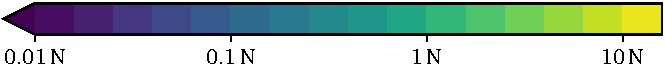
\includegraphics{biomech2ErrorForce_7}%
  \\[2mm]%
  \subcaptionbox{%
    $\abs{\forceXref - \forceXintp[p]}$ for
    $X = \mathrm{T}$ \emph{(left)} and
    $X = \mathrm{B}$ \emph{(right).}%
  }[74mm]{%
    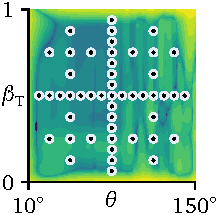
\includegraphics{biomech2ErrorForce_1}%
    \hfill%
    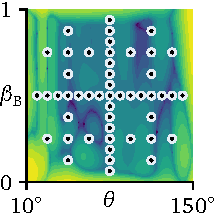
\includegraphics{biomech2ErrorForce_2}%
  }%
  \hfill%
  \subcaptionbox{%
    $\abs{\forceXref - \forceXintp[p,\cc]}$ for
    $X = \mathrm{T}$ \emph{(left)} and
    $X = \mathrm{B}$ \emph{(right).}%
  }[74mm]{%
    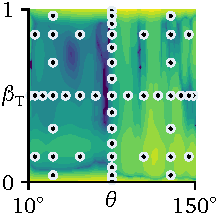
\includegraphics{biomech2ErrorForce_3}%
    \hfill%
    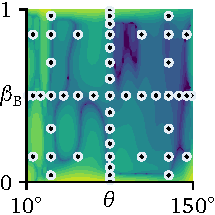
\includegraphics{biomech2ErrorForce_4}%
  }%
  \caption[Absolute error of muscle forces]{%
    Absolute error of muscle forces $\forceT, \forceB$ for
    modified cubic B-splines ($p = 3$)
    on sparse grids of uniform type \emph{(left two plots)} and
    of Clenshaw--Curtis type \emph{(right two plots)}
    together with the points of the sparse grid \emph{(dots).}%
  }%
  \label{fig:biomech2ErrorForce}%
\end{figure}

\pagebreak

\paragraph{Error of the equilibrium elbow angle}

The relative $\Ltwo$ errors
$\normLtwo{\equielbangref{\forceL} - \equielbangintp{\forceL}}/
\normLtwo{\equielbangref{\forceL}}$
of the equilibrium elbow angle function are shown in
\cref{tbl:biomech2ErrorL2_1} for the load of
$\forceL = \SI{22}{\newton}$.
Modified cubic Clenshaw--Curtis B-splines achieve the best results.
Therefore, we use this type of hierarchical basis
for the remainder of this chapter.
Pointwise plots of the absolute error
$\abs{\equielbangref{\forceL} - \equielbangintp[p,\cc]{\forceL}}$
are presented in \cref{fig:biomech2ErrorEquilibriumAngle}.
Again, the maximal error is comparatively small:
For $\forceL = \SI{22}{\newton}$, it is only \ang{0.886}.
If we restrict the domain to $\clint{0.15, 0.85}^2$,
then this maximal error drops to \ang{0.103} (or \ang{;6.18;}),
as the areas near the boundary of $\clint{\*0, \*1}$
contribute the most to the error.

\begin{figure}
  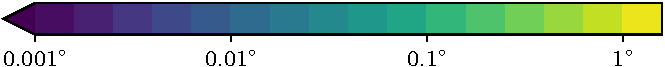
\includegraphics{biomech2ErrorEquilibriumAngle_5}%
  \\[2mm]%
  \subcaptionbox{%
    $\forceL = \SI{22}{\newton}$%
  }[49mm]{%
    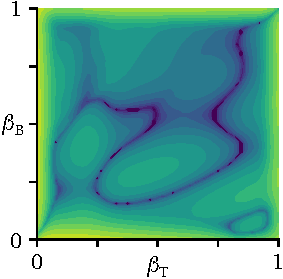
\includegraphics{biomech2ErrorEquilibriumAngle_1}%
  }%
  \hfill%
  \subcaptionbox{%
    $\forceL = \SI{-60}{\newton}$%
  }[49mm]{%
    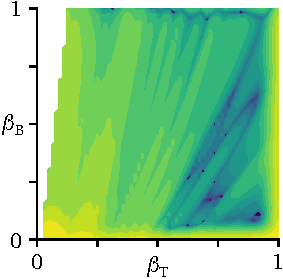
\includegraphics{biomech2ErrorEquilibriumAngle_2}%
  }%
  \hfill%
  \subcaptionbox{%
    $\forceL = \SI{180}{\newton}$%
  }[49mm]{%
    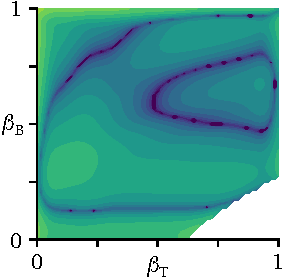
\includegraphics{biomech2ErrorEquilibriumAngle_3}%
  }%
  \caption[Absolute error of the equilibrium elbow angle]{%
    Absolute error
    $\abs{\equielbangref{\forceL} - \equielbangintp[p,\cc]{\forceL}}$
    of the equilibrium elbow angle for
    modified hierarchical cubic Clenshaw--Curtis B-splines ($p = 3$)
    for different loads $\forceL$.
    In the empty areas, at least one of
    $\equielbangref{\forceL}$ and $\equielbangintp[p,\cc]{\forceL}$
    is not well-defined (see \cref{eq:equilibriumAngle}).%
  }%
  \label{fig:biomech2ErrorEquilibriumAngle}%
\end{figure}



\subsection{Test Scenario}
\label{sec:734scenario}

\paragraph{Definition of the test scenario}

In the following, we want to assess the performance
of the sparse grid interpolants for the optimization problems
\ref{item:biomech2MinSum} and \ref{item:biomech2MinDist}.
For this goal, we create a test scenario \cite{Valentin18Gradient}
that simulates a pseudo-dynamic sequence of motions
by varying the load force and/or the target elbow angle
in discrete time steps $t$ as seen in \cref{fig:biomech2ScenarioA_1}.
The test scenario is as follows:
%
\begin{figure}
  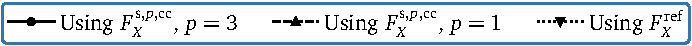
\includegraphics{biomech2ScenarioA_5}%
  \\[2mm]%
  \subcaptionbox{%
    Load $\forceL$ and target elbow angle $\tarelbang$.%
    \label{fig:biomech2ScenarioA_1}%
  }[73.3mm]{%
    \hspace*{4.5mm}%
    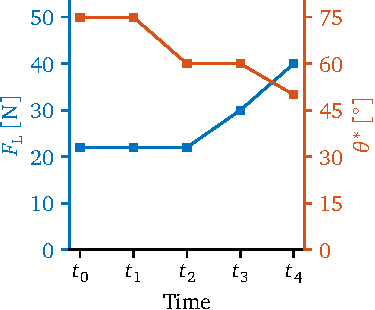
\includegraphics{biomech2ScenarioA_1}%
    \hspace*{2.4mm}%
  }%
  \hfill%
  \subcaptionbox{%
    Optimal activation parameters $\actT$ and $\actB$.%
    \label{fig:biomech2ScenarioA_2}%
  }[73.3mm]{%
    \hspace*{0.0mm}%
    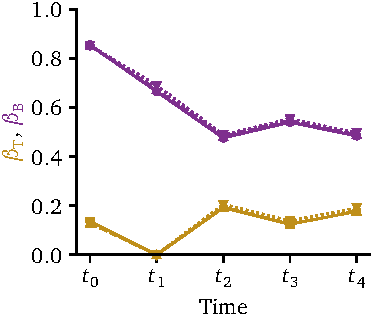
\includegraphics{biomech2ScenarioA_2}%
    \hspace*{9.8mm}%
  }%
  \\[1mm]%
  \subcaptionbox{%
    Deviation $\abs{\equielbang{\forceL} - \tarelbang}$
    of attained elbow angle to target and
    deviation \smash{$|\momentref|$} of the moment from equilibrium.%
    \label{fig:biomech2ScenarioA_3}%
  }[73.3mm]{%
    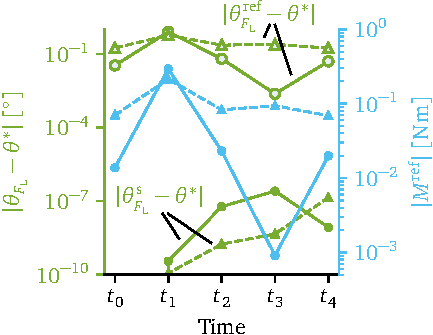
\includegraphics{biomech2ScenarioA_3}%
  }%
  \hfill%
  \subcaptionbox{%
    Number of evaluations of $\equielbang{\forceL}$
    and number of Newton iterations per evaluation
    of $\equielbang{\forceL}$.%
    \label{fig:biomech2ScenarioA_4}%
  }[73.3mm]{%
    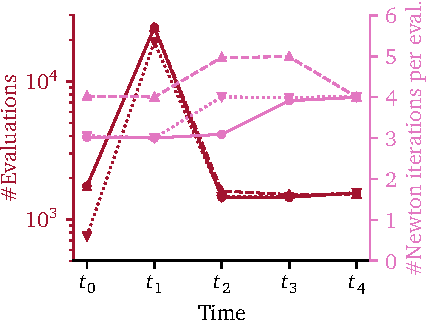
\includegraphics{biomech2ScenarioA_4}%
  }%
  \caption[Settings and results of the test scenario]{%
    Setting (a) of the test scenario and corresponding results (b, c, d).%
  }%
  \label{fig:biomech2ScenarioA}%
\end{figure}
%
\begin{enumerate}
  \item
  Find a feasible initial solution for problem \ref{item:biomech2MinSum}
  with $\forceL(t_0) \ceq \SI{22}{\newton}$ and
  $\tarelbang(t_0) \ceq \ang{75}$.
  
  \item
  Apply \ref{item:biomech2MinSum} with $\forceL(t_1) \ceq \SI{22}{\newton}$ and
  $\tarelbang(t_1) \ceq \ang{75}$.
  
  \item
  Apply \ref{item:biomech2MinDist} with $\forceL(t_2) \ceq \SI{22}{\newton}$ and
  $\tarelbang(t_2) \ceq \ang{60}$ (changed target angle).
  
  \item
  Apply \ref{item:biomech2MinDist} with $\forceL(t_3) \ceq \SI{30}{\newton}$ and
  $\tarelbang(t_3) \ceq \ang{60}$ (changed load).
  
  \item
  Apply \ref{item:biomech2MinDist} with $\forceL(t_4) \ceq \SI{40}{\newton}$ and
  $\tarelbang(t_4) \ceq \ang{50}$ (changed load and target angle).
\end{enumerate}
%
For each of the steps 2 to 5, the activation levels $\actT, \actB$ obtained
in the previous step (i.e., either the feasible initial solution
of step 1 or the optimal solution of steps 2 to 4) are used
as the input of the optimization problem
\ref{item:biomech2MinSum} or \ref{item:biomech2MinDist}.
The feasible initial solution in step 1 is determined as explained
in \cref{sec:513gradientBasedConstrained}.

\paragraph{Solutions of problem \ref{item:biomech2MinSum}}

We note that independently of $\forceL$ and $\tarelbang$,
every solution $(\actT, \actB)$ of problem \ref{item:biomech2MinSum} will be
on the boundary part of the domain $\clint{\*0, \*1}$,
on which at least one activation parameter vanishes, i.e.,
\begin{equation}
  \{(\actT, \actB) \in \clint{\*0, \*1} \mid
  (\actT = 0) \lor (\actB = 0)\}.
\end{equation}
The reason is that the two muscles triceps and biceps are antagonistic
(see \cref{sec:711models}), meaning that they work against each other.
If both $\actT > 0$ and $\actB > 0$, then the body will waste energy,
as the same target elbow angle can be attained by reducing both
$\actT$ and $\actB$ simultaneously, thus requiring less energy.
A visual example for this is \cref{fig:biomech2ReferenceEquilibriumAngle},
where the contour lines generally go from the bottom left
(small $\actT, \actB$) to the top right (large $\actT, \actB$).
This issue may be prevented by either
more complicated musculoskeletal models with more
than two muscles or different optimization problems
such as problem \ref{item:biomech2MinDist},
where the objective function differs.

\paragraph{Plots of optimization results}

\Cref{fig:biomech2ScenarioA_2,fig:biomech2ScenarioA_3,fig:biomech2ScenarioA_4}
show the results of the test scenario using the muscle forces
$\forceXintp[p,\cc]$ obtained by interpolating with
modified hierarchical cubic Clenshaw--Curtis B-splines (solid lines, $p = 3$).
As comparison, we repeat the solution process
with the forces obtained by interpolating with the
corresponding hierarchical piecewise linear basis (dashed lines, $p = 1$) and
with the reference forces $\forceXref$ (dotted lines).
For the piecewise linear basis,
we use exactly the same method as for the cubic case
(Newton method for $\equielbangintp{\forceL}$,
Augmented Lagrangian with adaptive gradient descent for the
solution of problems \ref{item:biomech2MinSum} and \ref{item:biomech2MinDist}),
although the derivatives of the muscle forces are discontinuous.
For the reference forces, we use the fact that the reference surrogates
are full grid spline interpolants, which can be explicitly differentiated.
Without the full grid interpolants,
we would have to approximate the derivatives with finite differences.

\vspace*{\fill}
\pagebreak

\paragraph{Equilibrium elbow angle}

In \cref{fig:biomech2ScenarioA_2}, we see that the activation levels
of all three methods are more or less the same.
However, \cref{fig:biomech2ScenarioA_3} reveals that even these small
differences lead to deviations of the resulting equilibrium elbow angle
to the target angle that differ by up to two orders of magnitude.
The two green lines with filled markers at the bottom of
\cref{fig:biomech2ScenarioA_3} show the error of
the equilibrium elbow angle $\equielbangintp{\forceL}$
using sparse grid interpolation to the desired target angle $\tarelbang$.
Unsurprisingly, this error is very small as
it is minimized by the optimizer as part of the constraint.
The true error, which is obtained by
using the reference equilibrium elbow angle $\equielbangref{\forceL}$,
is in general much larger
(top two green lines in \cref{fig:biomech2ScenarioA_3}
with hollow markers).
We see that the cubic B-splines decrease the error
by up to two orders of magnitude compared to the
piecewise linear basis.
There are two reasons for this:
First, the error of $\equielbang{\forceL}$ is generally smaller
when using higher-order B-splines as we have seen above.
Second, higher-order B-splines are continuously differentiable,
which makes them suitable for gradient-based optimization.
In contrast, the surrogates obtained by piecewise linear interpolation
have kinks, which may complicate finding optimal points
in the augmented Lagrangian and Newton methods.

\paragraph{Number of evaluations and Newton iterations}

This is supported by \cref{fig:biomech2ScenarioA_4},
which shows the number of evaluations of $\equielbang{\forceL}$
during the optimization and the average number of Newton iterations
per evaluation.
While the number of total evaluations is similar for all three methods,
the number of required Newton iterations to achieve convergence
is in general around \SI{50}{\percent} larger for the piecewise linear
basis functions.



\subsection{Spatial Adaptivity}
\label{sec:735adaptivity}

\paragraph{Generation of a spatially adaptive sparse grid}

As mentioned in \cite{Valentin18Gradient}, spatial adaptivity
may be employed to reduce the number of necessary muscle force samples
even further,
especially for more complicated musculoskeletal systems with
more parameters.
To verify this statement, we remove all grid points
$(\elbang^{(k,\cc)}, \actX^{(k,\cc)})$
from the regular sparse Clenshaw--Curtis grid that satisfy
\begin{equation}
  \frac{
    \abs{\alpha_\mathrm{T}^{(k,p,\cc)}}
  }{
    \max_{k'} \abs{\alpha_\mathrm{T}^{(k',p,\cc)}}
  } < \SI{1}{\percent}
  \quad\text{and}\quad
  \frac{
    \abs{\alpha_\mathrm{B}^{(k,p,\cc)}}
  }{
    \max_{k'} \abs{\alpha_\mathrm{B}^{(k',p,\cc)}}
  } < \SI{1}{\percent},
\end{equation}
where $\alpha_X^{(k,p,\cc)}$ ($X \in \{\mathrm{T}, \mathrm{B}\}$)
is the hierarchical surplus of the basis function $\bspl[\cc,\modified]{k}{p}$
corresponding to $(\elbang^{(k,\cc)}, \actX^{(k,\cc)})$.
For higher-dimensional models,
one would of course not sample muscle data on a regular sparse grid
and then coarsen the data by removing points,
but rather use an a posteriori adaptivity criterion to
decide which grid points to refine iteratively.

\paragraph{Comparison with the regular case}

For the cubic case $p = 3$,
the resulting force interpolants $\forceXintp[p,\cc,\mathrm{adap}]$ together
with the spatially adaptive sparse grid
(which has been coarsened from 49 to 28 points) and
equilibrium elbow angle $\equielbangintp[p,\cc,\mathrm{adap}]{\forceL}$
for $\forceL = \SI{22}{\newton}$ are shown in
\cref{fig:biomech2SpatiallyAdaptive}.
The sparse grid is almost dimensionally adaptive,
as $\forceXref$ seems to be almost linear in the $\actX$ direction
for both $X = \mathrm{T}$ and $X = \mathrm{B}$.
The errors increase slightly:
The relative $\Ltwo$ force errors for $(\mathrm{T}, \mathrm{B})$ increase
from $(\SI{3.31}{\permille}, \SI{3.56}{\permille})$
to $(\SI{3.36}{\permille}, \SI{4.43}{\permille})$,
and the absolute $\Linfty$ errors increase
from $(\SI{10.6}{\newton}, \SI{9.51}{\newton})$
to $(\SI{12.3}{\newton}, \SI{9.57}{\newton})$.
In addition, the relative $\Ltwo$ and absolute $\Linfty$ errors
for $\equielbang{\forceL}$ increase
from \SI{2.83}{\permille} and \ang{0.886}
to \SI{4.12}{\permille} and \ang{1.09}, respectively.
While all these errors are somewhat larger than for the regular sparse grid,
they are still at an acceptable level,
but the number of necessary muscle force evaluations is halved compared
to the regular case.
Additionally, the solution of the test scenario doesn't change significantly
due to the similar errors of $\forceX$ and $\equielbang{\forceL}$.

\begin{figure}
  \hspace*{2mm}%
  \raisebox{0.2mm}{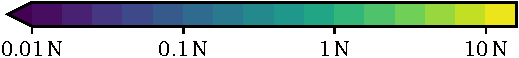
\includegraphics{biomech2ErrorForce_8}}%
  \hspace*{12mm}%
  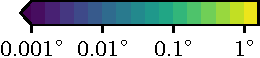
\includegraphics{biomech2ErrorEquilibriumAngle_6}%
  \\[2mm]%
  \subcaptionbox{%
    $\abs{\forceTref - \forceTintp[p,\cc,\mathrm{adap}]}$%
  }[49mm]{%
    \raisebox{1.02mm}{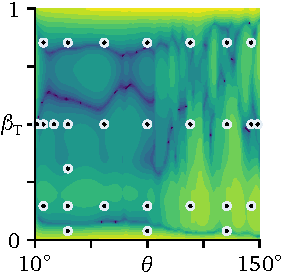
\includegraphics{biomech2ErrorForce_5}}%
  }%
  \hfill%
  \subcaptionbox{%
    $\abs{\forceBref - \forceBintp[p,\cc,\mathrm{adap}]}$%
  }[49mm]{%
    \raisebox{1.02mm}{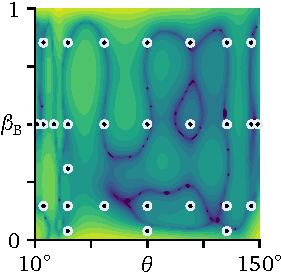
\includegraphics{biomech2ErrorForce_6}}%
  }%
  \hfill%
  \subcaptionbox{%
    $\abs{
      \equielbangref{\forceL} - \equielbangintp[p,\cc,\mathrm{adap}]{\forceL}
    }$
    for $\forceL = \SI{22}{\newton}$%
  }[49mm]{%
    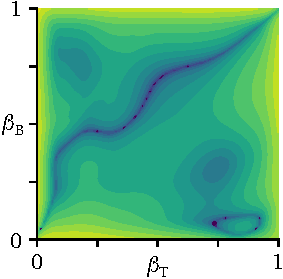
\includegraphics{biomech2ErrorEquilibriumAngle_4}%
  }%
  \caption[%
    Errors of muscle forces and equilibrium angle
    for the spatially adaptive case%
  ]{%
    Errors of muscle forces and equilibrium elbow angle
    for the spatially adaptive case
    (modified hierarchical cubic Clenshaw--Curtis B-splines,
    i.e., $p = 3$) together with the points of the
    spatially adaptive sparse grid \emph{(dots).}%
  }%
  \label{fig:biomech2SpatiallyAdaptive}%
\end{figure}
